\section{Grundlagen}
\subsection{Magnetooptischer Kerr-Effekt}
Der magneto-optische Kerr-Effekt (MOKE) beschreibt den Einfluss magnetischer Momente bei der Reflexion von Licht.
Er manifestiert sich in einer Drehung/"Anderung der Polarisation und Intensit"at des reflektierten Lichts.
Man unterscheidet prinzipiell zwischen drei Arten des MOKE, polarer, longitudinaler und transversaler MOKE.
Diese sind in Abbildung \ref{fig:moke_arten} gezeigt.
\begin{figure}[htpb]
    \centering
    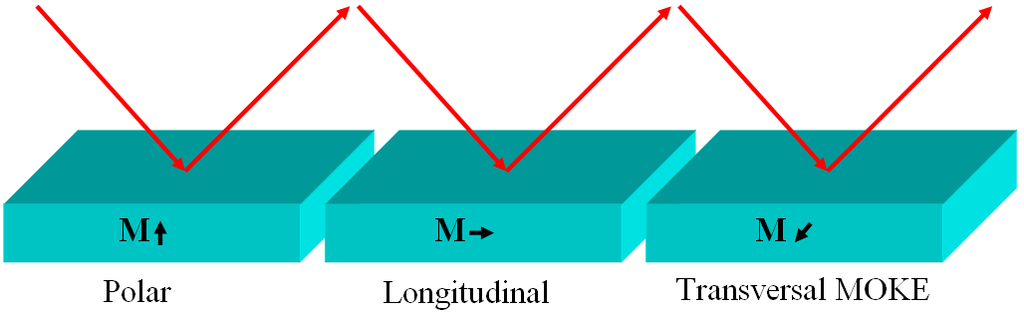
\includegraphics[width=0.8\textwidth]{../images/moke_arten.png}
    \caption{
        Die drei MOKE Arten: polar, longitudinal und transversal.
        Der Pfeil beschreibt die Richtung der magnetischen Polarisierung $M$ des Materials.
        Der blaue Pfeil zeigt Einfall und Reflexion des Lichts.\\
        Bild von: \url{https://upload.wikimedia.org/wikipedia/commons/thumb/b/b2/MOKE.PNG/1024px-MOKE.PNG}
        }
        \label{fig:moke_arten}
\end{figure}

F"ur die Anwendung bei optischen Speichermedien ist der polare MOKE (PMOKE) interessant.
Bei diesem ist die Magnetisierung senkrecht zur Oberfl"ache.
Bei diesem Effekt wird linear polarisiertes in elliptisch polarisiertes Licht umgewandelt und die Hauptachse wird um einen Winkel $\theta$ gedreht.
Erzeugt wird diese Drehung durch den sogenannten magnetisch zirkularen Dichroismus des Materials nach der Magnetisierung.
Dies bedeutet, dass es f"ur links und rechts zirkular polarisiertes Licht einen anderen Brechungsindex und Absorptionskoeffizienten hat.
Die beiden zirkularen Polarisationen erhalten daher eine andere Phasendifferenz und eine unterschiedliche Amplitude nach der Reflexion.
%TODO iclude a graphic
\cite{wikikerr}

\subsection{Optische Speichermedien}
\begin{figure}[htpb]
    \begin{minipage}[t][][t]{0.48\textwidth}
        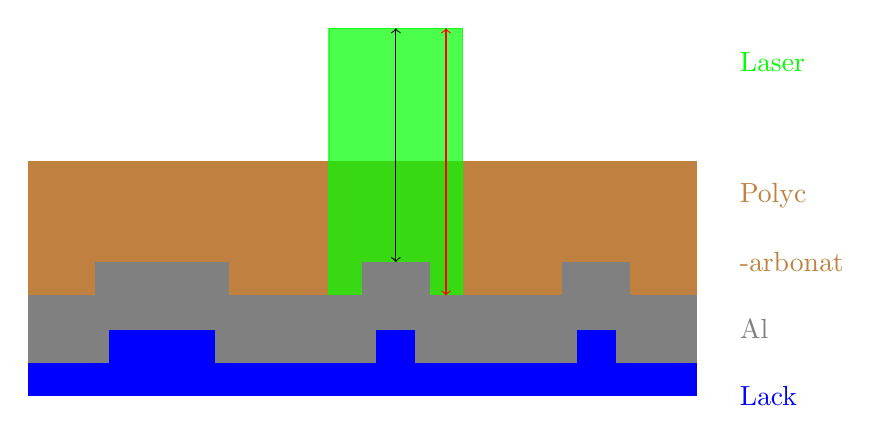
\begin{tikzpicture}
        [x=0.07\textwidth, y=0.07\textwidth]
        \draw[color=blue, fill=blue]
            (0,-0.5) rectangle (10,0.5)
            (10.5,-0.5) node[right]{Lack};
        \draw[color=brown, fill=brown]
            (0,1) rectangle (10,3)
            (10.5,2.5) node[right]{Polyc}
            (10.5,1.5) node[right]{-arbonat};
        \draw[color=green, fill=green, opacity=0.7]
            (4.5,1) rectangle (6.5,5);
        \draw[color=green, fill=green]
            (10.5,4.5) node[right]{Laser};
        \draw[color=gray, fill=gray]
            (0,0)--(0,1)--
            (1,1)--(1,1.5)--(3,1.5)--(3,1)--
            (5,1)--(5,1.5)--(6,1.5)--(6,1)--
            (8,1)--(8,1.5)--(9,1.5)--(9,1)--
            (10,1)--(10,0)--
            (8.8,0)--(8.8,0.5)--(8.2,0.5)--(8.2,0)--
            (5.8,0)--(5.8,0.5)--(5.2,0.5)--(5.2,0)--
            (2.8,0)--(2.8,0.5)--(1.2,0.5)--(1.2,0)--
            (0,0)
            (10.5,0.5) node[right]{Al};
        \draw[color=black, <->]
            (5.5,5)--(5.5,1.5);
        \draw[color=red, <->]
            (6.25,5)--(6.25,1);
        \end{tikzpicture}
        \caption{
            Schematische Zeichnung einer CD.
            Die reflektierende Aluminium Oberfl"ache enth"alt kleine Buckel (\SI{0.38}{\micro\metre} breit).
            Gesch"utzt wird sie durch eine Lackschicht und eine Polycarbonat-Schicht.
            Der Laser erfasst ein Gebiet welches gr"o{\ss}er ist, als der Buckel.
        }
        \label{fig:CD}
    \end{minipage}
    \hfill
    \begin{minipage}[t][][t]{0.48\textwidth}
        \begin{tikzpicture}
        [x=0.1\textwidth, y=0.1\textwidth]
        \draw[color=brown, fill=brown]
            (0,1) rectangle (7,2.5)
            (7.5,1.5) node[right]{Substrat};
        \draw[fill=gray]
            (0,0) rectangle (3,1)
            (4,0) rectangle (5,1)
            (6,0) rectangle (7,1);
        \draw[fill=brightgray]
            (3,0) rectangle (4,1)
            (5,0) rectangle (6,1);
        \draw[]
            (7.5,0.5) node[right]{MO-Schicht};
        \foreach \i in {.5,1.5,2.5,4.5,6.5} {
            \draw[fill=black, shift={(\i,0.5)}, opacity=0.8]
                (-0.1,-0.4)--(-0.1,0.2)--(-0.2,0.2)--(0,0.4)--(0.2,0.2)--(0.1,0.2)--(0.1,-0.4)--(-0.1,-0.4);
        }
        \foreach \i in {3.5,5.5} {
            \draw[fill=black, shift={(\i,0.5)}, opacity=0.8]
            (-0.1,0.4)--(-0.1,-0.2)--(-0.2,-0.2)--(0,-0.4)--(0.2,-0.2)--(0.1,-0.2)--(0.1,0.4)--(-0.1,0.4);
        }
        \draw[color=green, fill=green, opacity=0.5]
            (3,0) rectangle (4,4);
        \draw[color=green]
            (7.5,3.5) node[right]{Laser};
        \end{tikzpicture}
        \caption{
            Magneto Optical device (MO).
            Die Information ist in der MO-Schicht in Form von Spins gespeichert.
            Durch den Kerr-Effekt wird die Polarisation des reflektierten Lasers um den Winkel $\theta$ gedreht.
        }
        \label{fig:MO}
    \end{minipage}
\end{figure}
In optischen Speichermedien sind die Informationen auf einem Datentr"ager gespeichert, von dem sie mit Hilfe eines Lasers ausgelesen werden.

Ein Beispiel ist die CD oder CD-ROM, wo die Information bin"ar in Form von kleinen Buckeln auf einer reflektierenden Oberfl"ache gespeichert wird.
Ein Laser (Wellenl"ange $\lambda=\SI{780}{\nano\metre}$) rastert die Oberfl"ache der CD ab.
Wie in Abbildung \vref{fig:CD} gezeigt, trifft er dabei eine Fl"ache, die gr"o{\ss}er ist, als ein Buckel.
Trifft er nur auf Land (das ist der Bereich wo kein Buckel ist) so haben alle reflektierten Strahlen die gleiche Phase.
Trifft er aber auf einen Buckel, so legt der Laserstrahl eine k"urzere Strecke zur"uck.
Diese ist so gestaltet, das die Phasendifferenz zwischen schwarzem und rotem Lichtweg $\lambda/2$ betr"agt.
Durch destruktive Interferenz wird die reflektierte Intensit"at verringert. \cite{wikicd}

Eine weitere Form von optischen Speichermedien sind Magnetooptische Discs (MO).
Bei diesen wird die Information, wie in Abbildung \vref{fig:MO} dargestellt, in der lokalen Magnetisierung gespeichert.
Ausgelesen wird wiederum mit einem Laser, nur dass diesmal nicht Interferenz, sondern die Drehung der Polarisation um den Kerr-Winkel benutzt wird, um ein Bit zu speichern.
Eine MO kann beschrieben werden, indem ein Laser benutzt wird, um eine bestimmte Speicherposition aufzuheizen.
Dies senkt die magnetische Feldst"arke, die n"otig ist, um die Spins umzuklappen (Koerzitivfeldst"arke).
Durch anlegen eben jenes Magnetfeldes kann das Bit neu beschrieben werden.
Der Aufbau der Materialschichten einer MO ist in Abbildung \vref{fig:Struktur} gezeigt.
\cite{roll}
\begin{figure}[htbp]
    \begin{minipage}[t][][b]{0.48\textwidth}
        \centering
        \begin{tikzpicture}
        [x=0.8\textwidth,y=.15mm]
        \draw[fill=brown]
            (0,100)rectangle(1,200)
            (.5,150)node{Schutzschicht (\SI{10}{\micro\metre})};
        \draw[fill=white]
            (0,200)rectangle(1,260)
            (.5,230)node{Al (\SI{60}{nm})};
        \draw[fill=lightblue]
            (0,260)rectangle(1,310)
            (.5,285)node{SiN (\SI{50}{nm})};
        \draw[fill=brightgray]
            (0,310)rectangle(1,340)
            (.5,322.5)node{MO-Schicht (\SI{25}{nm})};
        \draw[fill=lightblue]
            (0,340)rectangle(1,395)
            (.5,365)node{SiN (\SI{110}{nm})};
        \draw[fill=brown]
            (0,395)rectangle(1,495)
            (.5,445)node{Polycarbonat Substrat (\SI{1.2}{mm})};
        \end{tikzpicture}
    \end{minipage}
    \begin{minipage}[t][][t]{0.48\textwidth}
        \caption{
            Aufbau einer MO.
            Das Zentrum bildet eine sehr d"unne magnetooptische Schicht, die von beiden Seiten durch SiN Schichten gegen Korrosion und Oxidation gesch"utzt wird.
            Die MO-Schicht ist typischerweise aus TbFeCo.
            Das Signal wird durch die reflektive Aluminiumschicht verst"arkt.
            Zus"atzlich wird die Disc noch durch eine Polykarbonat Schicht vor Besch"adigungen besch"utzt.
            \cite{roll}
        }
        \label{fig:Struktur}
    \end{minipage}
\end{figure}

\subsection{Stabilit"at Magnetooptischer Discs}
\begin{figure}[htbp]
    \begin{minipage}[t][][b]{0.48\textwidth}
        \centering
        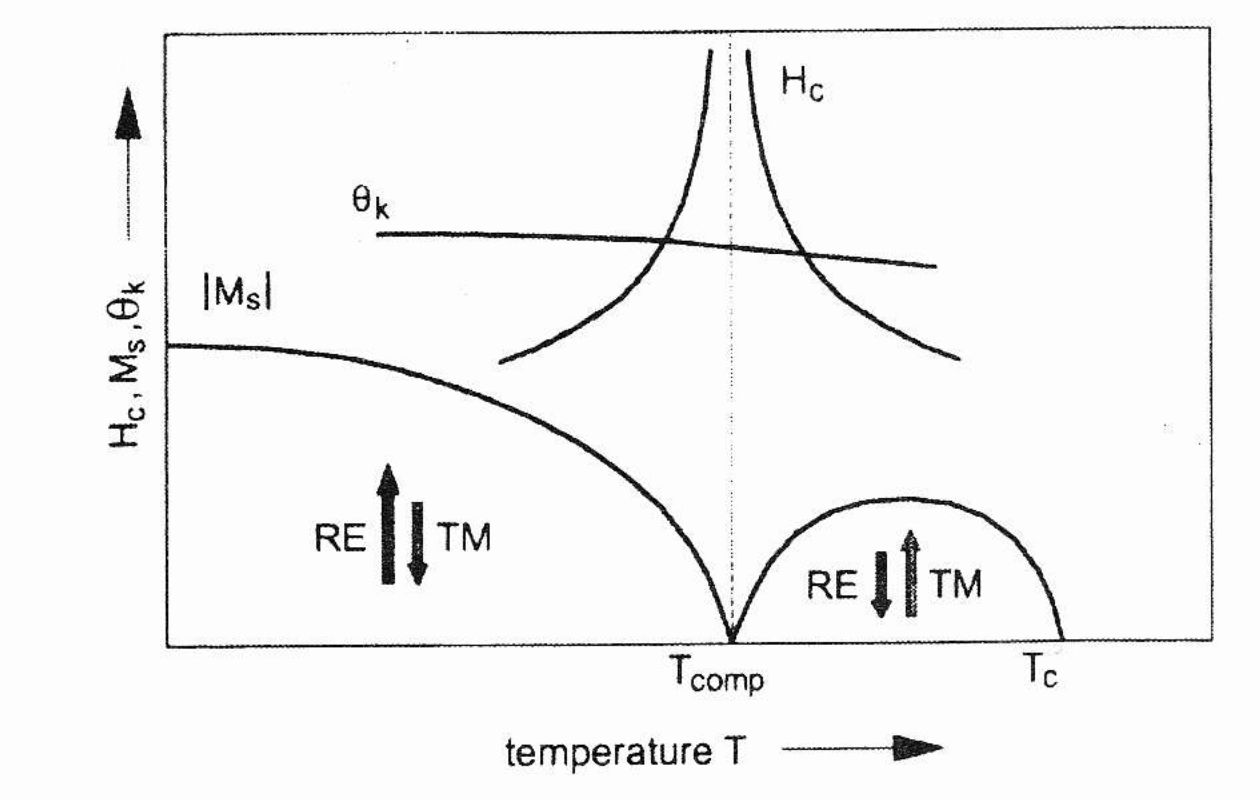
\includegraphics[width=\textwidth]{../images/temperatur.png}
    \end{minipage}
    \hfill
    \begin{minipage}[t][][t]{0.48\textwidth}
        \caption{
            Eigenschaften einer MO in Abh"angigkeit der Temperatur $T$.
            RE steht f"ur die seltenen Erde und TM f"ur das "Ubergangsmetall.
            Dabei ist $H_\text{c}$ die Koerzitivfeldst"arke, $M_\text{s}$ die totale Magnetisierung in Saturierung und $\theta_\text{K}$ der Kerr-Winkel.
            Zus"atzlich sind die Kompensationstemperatur $T_\text{comp}$ und die Curie Temperatur $T_\text{c}$ eingezeichnet.
            \cite{roll}
            }
        \label{fig:temperatur}
    \end{minipage}
\end{figure}
Wie funktioniert es eigentlich, dass eine MO bei Raumtemperatur nicht ummagnetisiert wird, wenn ein starker Magnet in die N"ahe kommt?
Die Antwort liegt im Material.
Es besteht aus zwei magnetischen Metallen, eine seltene Erde (RE) und ein "Ubergangsmetall (TM), die zusammen ein ferrimagnetisches Gitter bilden.
Zum Beispiel Tb und Fe.
Bei der Kompensationstemperatur $T_\text{comp}$ werden die Polarisierungen der beiden Metalle gleich stark und das Material antiferromagnetisch.
Wie in Abbildung \vref{fig:temperatur} zu sehen ist, divergiert f"ur diese Temperatur die Koerzitivfeldst"arke $H_\text{c}$ und das Material l"asst sich nicht mehr ummagnetisieren.
Nahe der kritischen Temperatur verh"alt sich die Koerzitivfeldst"arke wie
\begin{equation}
H_\mathrm{c} = \frac{H_0 \cdot T}{T-T_\mathrm{comp}},
\label{eq:Hc}
\end{equation}
wobei $H_0$ ein Proportionalit"atsfaktor ist.
Die gesamte Magnetisierung l"asst sich als die Summe zweier ferromagnetischer Magnetisierungskurven mit entgegengesetztem Vorzeichen und unterschiedlicher Curie Temperatur beschreiben.
Wie zu erkennen ist, "andert sich der Kerr-Winkel etwa linear mit der Temperatur, aber nur schwach.

Aber wenn die gesamte Magnetisierung bei Raumtemperatur null ist, wie wird dann gemessen.
Hier macht man sich zunutze, dass die Elektronenh"ullen der seltenen Erde, die die Magnetisierung tragen, weiter innen liegen, also durch "au{\ss}ere H"ullen abgeschirmt werden.
Das Licht wird also an nicht-magnetisierbaren Elektronenh"ullen gestreut.
Bei einem "Ubergangsmetall hingegen tragen die "au{\ss}eren H"ullen die Magnetisierung; diese streuen das Licht und die Magnetisierung wird wahrgenommen.
Der Laser sieht also nur das ferromagnetische Untergitter des "Ubergangsmetalls.
\cite{roll}


\subsection{Magnetisch Induzierte Super Aufl"osung (MSR)}
\begin{figure}[htbp]
    \begin{minipage}[t][][b]{0.48\textwidth}
        \centering
        \begin{tikzpicture}
            [x=0.1\textwidth, y=0.1\textwidth]
            \draw[color=brown, fill=brown]
                (0,2) rectangle (7,3.5)
                (7.5,2.5) node[right]{Substrat};
            \draw[fill=gray]
                (0,0) rectangle (3,1)
                (4,0) rectangle (5,1)
                (6,0) rectangle (7,1);
            \draw[fill=brightgray]
                (3,0) rectangle (4,1)
                (5,0) rectangle (6,1);
            \draw[fill=darkgray]
                (0,1) rectangle (3,2)
                (4,1) rectangle (7,2);
            \draw[fill=gray]
                (3,1) rectangle (4,2);
            \draw[]
                (7.5,0.5) node[right]{MO-Schicht}
                (7.5,1.5) node[right]{Lese Schicht}
                ;
            \foreach \i in {.5,1.5,2.5,4.5,6.5} {
                \draw[fill=black, shift={(\i,0.5)}, opacity=0.8]
                    (-0.1,-0.4)--(-0.1,0.2)--(-0.2,0.2)--(0,0.4)--(0.2,0.2)--(0.1,0.2)--(0.1,-0.4)--(-0.1,-0.4);
            }
            \foreach \i in {3.5,5.5} {
                \draw[fill=black, shift={(\i,0.5)}, opacity=0.8]
                    (-0.1,0.4)--(-0.1,-0.2)--(-0.2,-0.2)--(0,-0.4)--(0.2,-0.2)--(0.1,-0.2)--(0.1,0.4)--(-0.1,0.4);
            }
            \foreach \i in {.5,1.5,2.5,4.5,5.5,6.5} {
                \draw[fill=black, shift={(\i,1.5)}, opacity=0.8, rotate=-90]
                    (-0.1,-0.4)--(-0.1,0.2)--(-0.2,0.2)--(0,0.4)--(0.2,0.2)--(0.1,0.2)--(0.1,-0.4)--(-0.1,-0.4);
            }
            \foreach \i in {3.5} {
                \draw[fill=black, shift={(\i,1.5)}, opacity=0.8]
                    (-0.1,0.4)--(-0.1,-0.2)--(-0.2,-0.2)--(0,-0.4)--(0.2,-0.2)--(0.1,-0.2)--(0.1,0.4)--(-0.1,0.4);
            }
            \draw[color=green, fill=green, opacity=0.5]
                (2.5,0) rectangle (4.5,4);
            \draw[color=green]
                (7.5,3.5) node[right]{Laser};
        \end{tikzpicture}
    \end{minipage}
    \hfill
    \begin{minipage}[t][][t]{0.45\textwidth}
        \caption{
            Magnetisch induzierte super Aufl"osung (MSR).
            Zus"atzlich zur MO-Schicht gibt es jetzt auch noch eine Lese Schicht.
            Diese gleicht sich nur im AStrahlzentrum der MO-Schicht an.
        }
        \label{fig:MSR}
    \end{minipage}
\end{figure}

Der Laser trifft ein bestimmtes Gebiet, was die Gr"o{\ss}e eines Bits definiert.
Um die Aufl"osung zu erh"ohen kann ein zweites magnetooptisches Material "uber die MO-Schicht gelegt werden, wie in Abbildung \vref{fig:MSR} gezeigt wird.
Dieses wird durch den Laser aufgeheizt und dadurch magnetisierbar.
Allerdings geschieht dies nur im Strahlzentrum, also auf einem Bereich, der kleiner ist, als der Laser.
Dieser kleine Bereich der Lese Schicht passt sich dann der Magnetisierung der MO-Schicht an und kann ausgelesen werden.
\cite{roll}


